% 第 4 章
\section{Gradient Descent 优化视角：迭代、不动点与精确解}\label{sec:gd}

第 \ref{sec:hd-closed} 节给出了闭式解 $\bhat = (\X^\top\X)^{-1}\X^\top\y$，但「能写出来」不等于「该直接算」：显式求逆要解 $d \times d$ 线性方程组，代价约 $O(d^3)$，且形成 $\X^\top\X$ 会把 $\X$ 的条件数平方。这一章换到优化的视角：不直接解正规方程，而是从某个初值 $\widehat{\bbeta}_0$ 出发，让损失函数自己「下山」。我们会看到——\textbf{由于损失是二次的，这条下山路线可以被精确地写出来}：$\widehat{\bbeta}_t$ 有关于 $t$、$\X$、$\y$ 的闭式表达，而且它恰好以闭式解 $\bhat$ 为不动点。

\subsection{梯度下降迭代与不动点}\label{sec:gd-iter}

取约定（机器学习中的标准写法）
\begin{equation}\label{eq:gd-loss}
  L(\bbeta) = \frac{1}{2}\norm{\y - \X \bbeta}^2,
  \qquad
  \nabla L(\bbeta) = \X^\top (\X \bbeta - \y),
\end{equation}
（$\frac12$ 只是约定，使梯度没有因子 $2$；若坚持用 $L = \norm{\cdot}^2$，下文所有 $\eta$ 换成 $2\eta$ 即可。）注意你写的迭代式
\[
  \widehat{\bbeta}_{t+1} = \widehat{\bbeta}_t - \eta\, L(\widehat{\bbeta}_t)
\]
需要一个小的修正：$L$ 是标量，标量不能从向量里减掉——下山方向是\textbf{梯度的负方向}，$\eta > 0$ 是步长（learning rate）。迭代为
\begin{equation}\label{eq:gd}
  \boxed{\;\widehat{\bbeta}_{t+1} = \widehat{\bbeta}_t - \eta\, \nabla L(\widehat{\bbeta}_t)
       = \widehat{\bbeta}_t - \eta\, \X^\top \big( \X \widehat{\bbeta}_t - \y \big)\;}
\end{equation}

\textbf{不动点}（fixed point）是满足「迭代一步后不再移动」的点：
\begin{equation}\label{eq:fixed}
  \bbeta^\star = \bbeta^\star - \eta\, \nabla L(\bbeta^\star)
  \quad\Longleftrightarrow\quad
  \nabla L(\bbeta^\star) = \zero
  \quad\Longleftrightarrow\quad
  \X^\top \X \, \bbeta^\star = \X^\top \y .
\end{equation}
不动点条件就是正规方程！因此当 $\X$ 列满秩、$0 < \eta < \infty$ 时，\eqref{eq:gd} 有唯一不动点
\begin{equation}\label{eq:gd-fixed}
  \boxed{\;\bbeta^\star = (\X^\top \X)^{-1} \X^\top \y = \bhat\;}
\end{equation}
——梯度下降与最小二乘是同一个对象的两条路径：\textit{一条直接解方程（第 \ref{sec:hd-closed} 节），一条迭代逼近（本节），而它们共享同一个终点。}这正是「把两个公式放在一起」的第一层含义。

\subsection[把两个公式放在一起：迭代解的精确解]{把两个公式放在一起：$\widehat{\bbeta}_t$ 的精确解}\label{sec:gd-exact}

现在做第二层：把 \eqref{eq:gd} 与 \eqref{eq:gd-fixed} 联立，写出\textbf{任意时刻 $t$ 的精确解}。

把 \eqref{eq:gd} 改写成「误差传播」形式。记 $\bm{A} := \bm{I} - \eta \X^\top \X$，注意不动点给出
\[
  \eta\, \X^\top \y = \eta\, \X^\top \X \bbeta^\star = (\bm{I} - \bm{A})\, \bbeta^\star .
\]
代入 \eqref{eq:gd}：
\[
  \widehat{\bbeta}_{t+1} = (\bm{I} - \eta \X^\top\X)\, \widehat{\bbeta}_t + \eta \X^\top \y
  = \bm{A}\, \widehat{\bbeta}_t + (\bm{I} - \bm{A})\, \bbeta^\star,
\]
即
\[
  \widehat{\bbeta}_{t+1} - \bbeta^\star = \bm{A}\, \big( \widehat{\bbeta}_t - \bbeta^\star \big).
\]
误差向量每步左乘同一个矩阵 $\bm{A}$——线性迭代的全部秘密就藏在这一行里。递推 $t$ 次：

\begin{theorem}[$\widehat{\bbeta}_t$ 的精确解]\label{thm:gd-exact}
对任意初值 $\widehat{\bbeta}_0$ 与任意 $t \ge 0$，
\begin{equation}\label{eq:gd-exact}
  \boxed{\;\widehat{\bbeta}_t = \underbrace{(\X^\top \X)^{-1} \X^\top \y}_{\bhat}
  + \big( \bm{I} - \eta\, \X^\top \X \big)^{t}\; \big( \widehat{\bbeta}_0 - (\X^\top \X)^{-1} \X^\top \y \big)\;}
\end{equation}
即「闭式解 + 初始误差的 $t$ 次幂衰减」。特别地，取 $\widehat{\bbeta}_0 = \zero$（最常见的默认）：
\begin{equation}\label{eq:gd-exact-zero}
  \widehat{\bbeta}_t = \Big[ \bm{I} - \big( \bm{I} - \eta\, \X^\top \X \big)^{t} \Big] (\X^\top \X)^{-1} \X^\top \y .
\end{equation}
\end{theorem}
\begin{proof}
\eqref{eq:gd-exact} 由 $\widehat{\bbeta}_t - \bbeta^\star = \bm{A}^t (\widehat{\bbeta}_0 - \bbeta^\star)$ 展开即得，后者由上面的误差递推归纳 $t$ 步（$t=0$ 时 $\bm{A}^0 = \bm{I}$ 显然成立）。\eqref{eq:gd-exact-zero} 代入 $\widehat{\bbeta}_0 = \zero$ 并用 $\bbeta^\star = \bhat$。
\end{proof}

这个精确解把三件事讲透了：

\begin{enumerate}[label=(\arabic*)]
  \item \textbf{收敛与否完全由 $\bm{I} - \eta\X^\top\X$ 的特征值决定}。设 $\X^\top\X$ 的特征值为 $\lambda_1 \ge \dots \ge \lambda_d > 0$（列满秩保证全正），则 $\bm{A}$ 的特征值为 $1 - \eta \lambda_j$。误差沿特征方向 $\bm{v}_j$ 以因子 $(1 - \eta\lambda_j)^t$ 衰减。
  \item \textbf{$t \to \infty$ 时收敛到 $\bhat$ 的充要条件是} 所有方向都收缩：
  \begin{equation}\label{eq:gd-conv}
    \big| 1 - \eta \lambda_j \big| < 1 \ \ \forall j
    \quad\Longleftrightarrow\quad
    \boxed{\;0 < \eta < \frac{2}{\lambda_{\max}(\X^\top\X)}\;}
  \end{equation}
  步长太大（$\eta \ge 2/\lambda_{\max}$）时，最大特征值方向发散，迭代爆炸——「learning rate 不能太大」第一次有了精确的代数含义。
  \item \textbf{梯度下降在「近似求逆」}。当 $\eta < 1/\lambda_{\max}$ 时 $\norm{\bm{A}} < 1$，有几何级数（Neumann 级数）
  \[
    \eta \sum_{k=0}^{t-1} \bm{A}^k = \eta \sum_{k=0}^{t-1} (\bm{I} - \eta \X^\top \X)^k
    \;\xrightarrow[t \to \infty]{}\; (\X^\top \X)^{-1},
  \]
  因此 \eqref{eq:gd-exact-zero} 正是「用 $t$ 项多项式逼近 $(\X^\top\X)^{-1}$」。闭式解一步到位地求逆；梯度下降用迭代多项式一部部地拼出逆——同一个 $(\X^\top\X)^{-1}$，一个直给，一个按揭。
\end{enumerate}

\subsection{步长的最优选择与条件数的阴影}\label{sec:gd-rate}

在收敛区间 \eqref{eq:gd-conv} 内，最慢方向决定速度：渐近收敛率由 $\max_j |1 - \eta \lambda_j|$ 给出。最优步长让两端的衰减因子相等：

\begin{corollary}[最优步长与收敛率]\label{thm:gd-opt}
记 $\lambda_{\min}, \lambda_{\max}$ 为 $\X^\top\X$ 的最小、最大特征值，条件数 $\kappa = \lambda_{\max}/\lambda_{\min}$。最优步长与对应渐近收敛率为
\begin{equation}\label{eq:gd-opt}
  \eta^\star = \frac{2}{\lambda_{\min} + \lambda_{\max}},
  \qquad
  \rho^\star = \max_j |1 - \eta^\star \lambda_j| = \frac{\kappa - 1}{\kappa + 1} < 1 .
\end{equation}
\end{corollary}
\begin{proof}
$\max_j |1 - \eta\lambda_j| = \max\{|1 - \eta\lambda_{\min}|, |1 - \eta\lambda_{\max}|\}$。在收敛区间内前者随 $\eta$ 减、后者随 $\eta$ 增，最优在 $1 - \eta\lambda_{\min} = \eta\lambda_{\max} - 1$ 处取得，解出 $\eta^\star$；代入即得 $\rho^\star = (\lambda_{\max} - \lambda_{\min})/(\lambda_{\max} + \lambda_{\min})$。
\end{proof}

\textbf{步长的三档分野。}把 $\eta$ 按它与谱端点 $1/\lambda_{\max}$、$2/\lambda_{\max}$ 的关系分成三档。三档的分界在\textbf{迭代轨道}上看最清楚（图 \ref{fig:ch4-gd}），在标量上看则是带符号误差的三种形态（图 \ref{fig:ch4-loss}）：

\begin{enumerate}[label=第\arabic*档：, leftmargin=3.2em]
  \item \textbf{$0 < \eta \le 1/\lambda_{\max}$，单调下降。}此时所有特征值满足 $0 \le 1 - \eta\lambda_j < 1$：每个方向的误差因子都非负，迭代朝 $\bhat$ 直线前进，误差投影不变号、损失一步不回头（图 \ref{fig:ch4-loss}(a)）。这一档最安全，但最慢——按最小特征方向计，每步只压缩 $1 - \eta\lambda_{\min}$，大步长被最大特征值锁死，只能委曲求全。
  \item \textbf{$1/\lambda_{\max} < \eta < 2/\lambda_{\max}$，轨道震荡、损失仍降。}步长越过第一档边界后，最大特征方向上的因子 $1 - \eta\lambda_{\max}$ 变负：迭代每步在谷底两侧\textbf{过冲、翻号}——图 \ref{fig:ch4-gd}(b) 的之字轨、图 \ref{fig:ch4-loss}(b) 中带符号误差的锯齿都源于此。但请注意一个常被忽略的事实：\emph{损失本身并不震荡}。由 \eqref{eq:gd-exact}，
  \[
    L(\widehat{\bbeta}_t) - L_{\min}
    = \frac12 \sum_{j=1}^{d} \lambda_j \big( 1 - \eta \lambda_j \big)^{2t} c_j^2,
    \qquad c_j = \bm{v}_j^\top \big( \widehat{\bbeta}_0 - \bhat \big),
  \]
  每一项都是\emph{偶次幂}——翻号在平方里被消灭了，损失曲线依旧单调下滑（图 \ref{fig:ch4-loss}(b) 灰虚线）。\textbf{震荡的是轨道，不是损失。}只要 $|1 - \eta\lambda_{\max}| < 1$，锯齿幅度就持续衰减，震荡不等于发散。耐人寻味的是，最优步长 $\eta^\star = 2/(\lambda_{\min} + \lambda_{\max})$ 恰好落在这一档（当 $\kappa > 1$ 时 $1/\lambda_{\max} < \eta^\star < 2/\lambda_{\max}$）：\emph{最快的策略不是小心翼翼地不回头，而是允许自己在最长方向上适度过冲，用翻号换取整体的最速衰减}。
  \item \textbf{$\eta \ge 2/\lambda_{\max}$，震荡不收敛。}因子 $|1 - \eta\lambda_{\max}| \ge 1$，最大特征方向每步翻号且幅度不再衰减（等号时锯齿永不消失）：轨道呈发散之字（图 \ref{fig:ch4-gd}(c)），带符号误差与损失同步爆炸，数步之内溢出（图 \ref{fig:ch4-loss}(c)）。
\end{enumerate}

三档的边界 $1/\lambda_{\max}$ 与 $2/\lambda_{\max}$ 都只依赖最大特征值——这正是工程上「learning rate 调太大就 nan」的精确代数解释；而三档之内「快与稳」的权衡由条件数 $\kappa$ 裁决。

\begin{figure}[htbp]
  \centering
  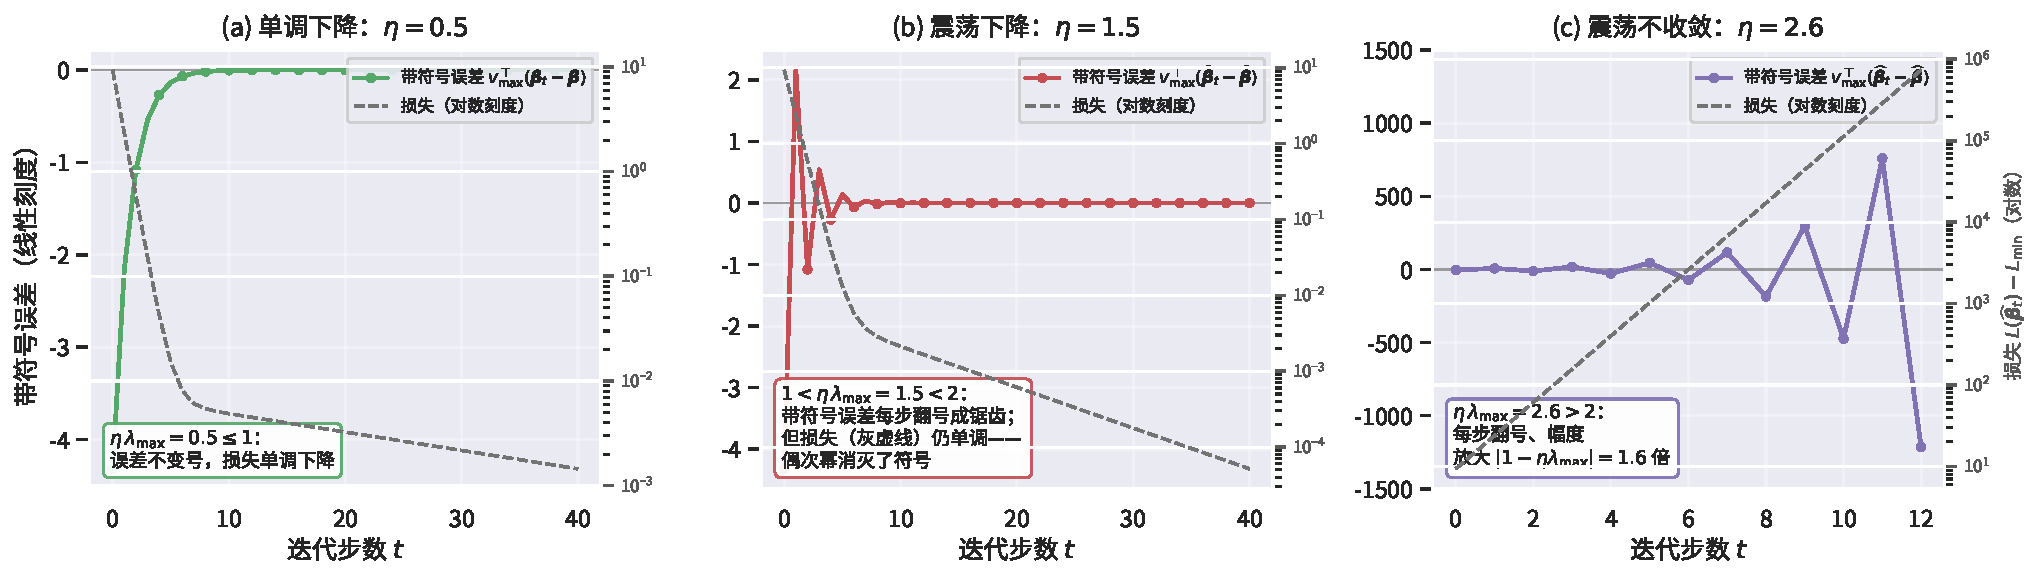
\includegraphics[width=\linewidth]{figures/ch4_loss.pdf}
  \caption{带符号误差（彩色实线，左轴，线性刻度）与损失（灰虚线，右轴，对数刻度）随迭代步数 $t$ 的三档形态（同一二次问题、同一初值、仅改变 $\eta$）：(a) 单调下降——$\eta\lambda_{\max} \le 1$，最大特征方向误差不变号，损失单调；(b) 震荡下降——$1 < \eta\lambda_{\max} < 2$，带符号误差每步翻号成锯齿，但损失因偶次幂仍单调下滑；(c) 震荡不收敛——$\eta\lambda_{\max} > 2$，误差每步翻号、幅度以 $|1-\eta\lambda_{\max}|$ 倍放大，损失爆炸。}
  \label{fig:ch4-loss}
\end{figure}

两个实践推论，都是「为什么学线性回归」的答案碎片：

\begin{itemize}
  \item \textbf{条件数统治一切。}$\kappa \approx 1$（特征方向长短一致）时 $\rho^\star \approx 0$，几步收敛；$\kappa \gg 1$（第 \ref{sec:hd-break} 节的病态）时 $\rho^\star \approx 1 - 2/\kappa$，收敛以 $O(\kappa \log(1/\varepsilon))$ 步计——\textit{与特征缩放强相关的工程经验「先标准化特征」}，在这里是半个定理：标准化把 $\X^\top\X$ 的对角元归一，\textbf{消除了条件数中由量纲差异贡献的部分}——但由\textbf{相关结构}（共线）造成的特征值分散完全不受影响，$\kappa$ 仍可以很大。
  \item \textbf{预处理 = 坐标变换下的 GD。}对 $\X^\top\X$ 做谱分解后做白化，等价于在更好的坐标系里跑梯度下降；共轭梯度法（CG）则可视为「每步自动选步长与方向的 GD」，$d$ 步内\textbf{精确}到达 $\bhat$（二次函数的有限终止性）。从 GD 到 CG 到直接求逆，是一个谱系，两端是「迭代 $t$ 步」与「闭式一步」，中间全是同一几何的插值。
\end{itemize}

\begin{figure}[htbp]
  \centering
  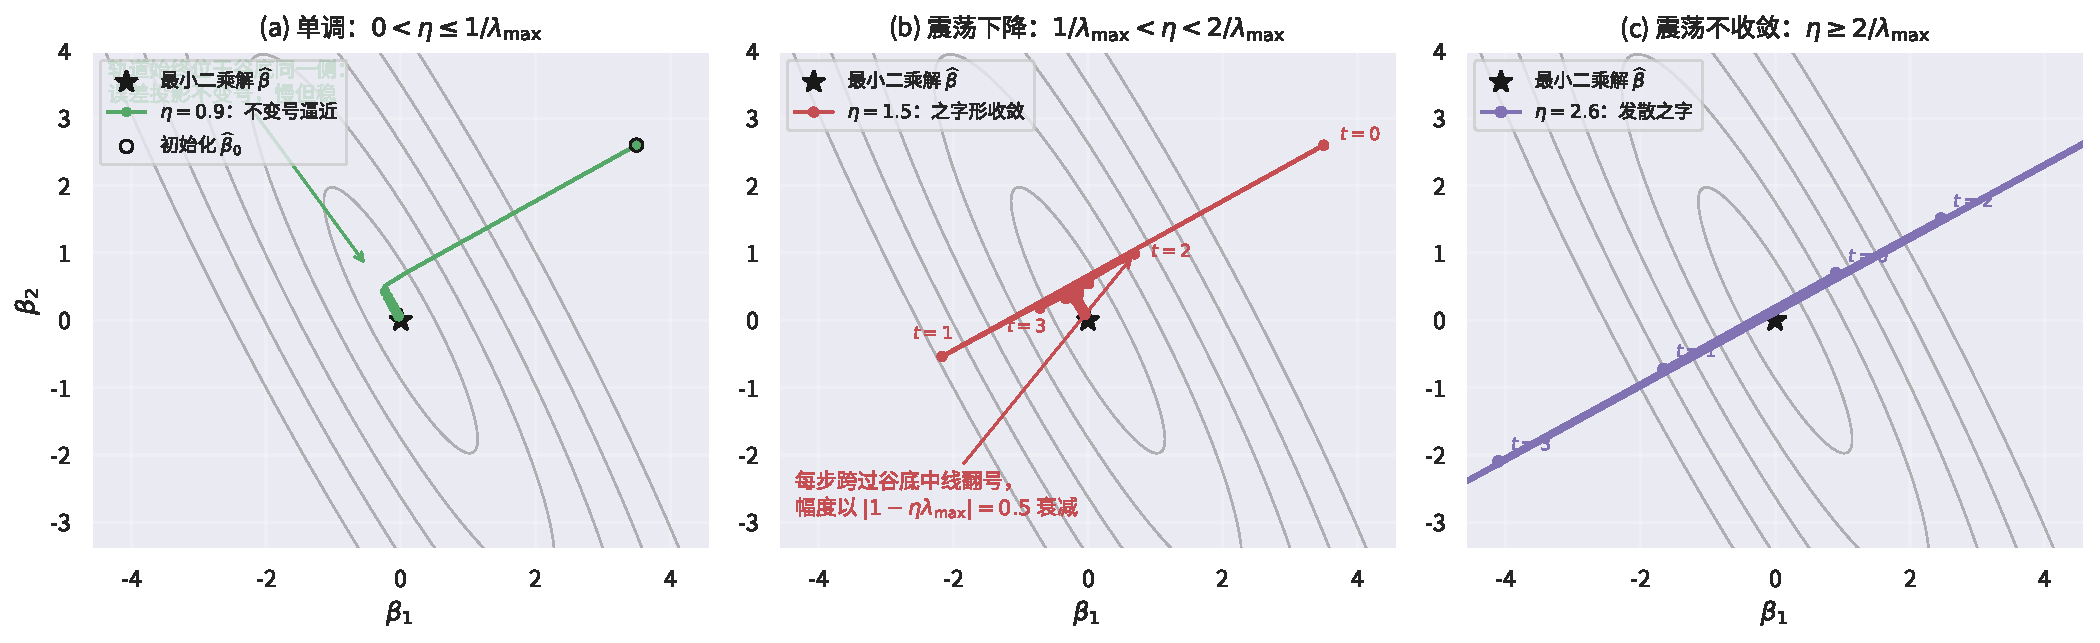
\includegraphics[width=\linewidth]{figures/ch4_gd.pdf}
  \caption{梯度下降在二次损失（条件数 $\kappa=25$ 的椭圆谷）上的三条轨道，与步长三档一一对应：(a) $\eta=0.9 \le 1/\lambda_{\max}$：轨道不跨谷底中线、不变号逼近，但沿「瘦」方向缓慢爬行；(b) $1/\lambda_{\max}<\eta=1.5<2/\lambda_{\max}$：轨道每步跨过谷底翻号，之字形幅度以 $|1-\eta\lambda_{\max}|=0.5$ 衰减——震荡下降；(c) $\eta=2.6>2/\lambda_{\max}$：每步翻号、幅度放大 $1.6$ 倍，数步内飞出视野。}
  \label{fig:ch4-gd}
\end{figure}

\subsection{与闭式解的对照表}

\begin{center}
\begin{tabular}{@{}lll@{}}
\toprule
 & 闭式解 $\bhat = (\X^\top\X)^{-1}\X^\top\y$ & 梯度下降 \eqref{eq:gd} \\
\midrule
性质 & 一步到位（解 $d\times d$ 系统） & 逐步逼近，$t$ 步后误差 $\propto \rho^t$ \\
代价（列满秩） & $O(nd^2 + d^3)$，须形成 $\X^\top\X$ & 每步 $O(nd)$ 矩阵向量乘，内存友好 \\
适用区域 & $n \gg d$ 的经典区间 & 任意 $n, d$（配合正则化/早期停止） \\
病态 $\kappa \gg 1$ & 数值不稳定（条件数平方） & 收敛极慢（同样的 $\kappa$，不同的病法） \\
与 $\bhat$ 的关系 & 就是它 & 不动点即 $\bhat$；$\widehat{\bbeta}_t$ 有精确解 \eqref{eq:gd-exact} \\
\bottomrule
\end{tabular}
\end{center}

\begin{keybox}[本章要点]
\begin{itemize}
  \item 梯度下降迭代 $\widehat{\bbeta}_{t+1} = \widehat{\bbeta}_t - \eta\,\X^\top(\X\widehat{\bbeta}_t - \y)$ 的不动点条件 $\nabla L = \zero$ 就是正规方程，唯一不动点即闭式解 $\bhat$——优化视角与代数视角终点相同；
  \item 联立两式得精确解 $\widehat{\bbeta}_t = \bhat + (\bm{I} - \eta\X^\top\X)^t(\widehat{\bbeta}_0 - \bhat)$：误差每步左乘 $\bm{I} - \eta\X^\top\X$，特征值 $1 - \eta\lambda_j$ 决定各方向衰减；
  \item 收敛当且仅当 $0 < \eta < 2/\lambda_{\max}$；最优 $\eta^\star = 2/(\lambda_{\min} + \lambda_{\max})$，渐近率 $(\kappa - 1)/(\kappa + 1)$——「标准化特征」消除量纲导致的病态（相关结构导致的病态它无能为力）；
  \item GD 的几何级数形式说明它在用 $t$ 次多项式逼近 $(\X^\top\X)^{-1}$：闭式解直给逆，迭代解按揭逆；共轭梯度是谱系的中点。
\end{itemize}
\end{keybox}

\begin{exercise}\label{ex:gd-rate}
由 \eqref{eq:gd-exact} 推导：若 $\widehat{\bbeta}_0 = \zero$ 且 $\eta = \eta^\star$，则 $\norm{\widehat{\bbeta}_t - \bhat} \le \big(\frac{\kappa-1}{\kappa+1}\big)^t \norm{\bhat}$；并由此给出达到 $\norm{\widehat{\bbeta}_t - \bhat} \le \varepsilon$ 所需步数的 $O(\cdot)$ 表达式。
\end{exercise}

\begin{exercise}\label{ex:neumann}
验证恒等式 $\eta\sum_{k=0}^{t-1}(\bm{I} - \eta\X^\top\X)^k \X^\top\y = \big[\bm{I} - (\bm{I} - \eta\X^\top\X)^t\big]\bhat$（提示：两边同乘 $\X^\top\X$ 或用 Neumann 级数），说明它正是 \eqref{eq:gd-exact-zero} 的左乘形式。
\end{exercise}
